%%%%%%%%%%%%%%%%%%%%%%%%%%%%%%%%%%%%%%%%%%%%%%%%%%%%%%%%%%%%%%%%%
%                                                               %
%        encodage : utf8                                        %
%                                                               %
%%%%%%%%%%%%%%%%%%%%%%%%%%%%%%%%%%%%%%%%%%%%%%%%%%%%%%%%%%%%%%%%%
%                                                               %
%           耿楠 2019/01/01                                     %
%  Copyright (c) 2019 __耿楠__ All rights reserved.             %
%        version : 1.0                                          %
% 该代码改自于:https://github.com/tkz-sty/tkz-kiviat            %
%%%%%%%%%%%%%%%%%%%%%%%%%%%%%%%%%%%%%%%%%%%%%%%%%%%%%%%%%%%%%%%%%
% This file may be distributed and/or modified
%
% 1. under the LaTeX Project Public License , either version 1.3
% of this license or (at your option) any later version and/or
% 2. under the GNU Public License.
% See http://www.latex-project.org/lppl.txt for details.    
% graphs from graph theory

\documentclass[DIV         = 12,
               fontsize    = 10,
               headinclude = false,
               index       = totoc,
               footinclude = false,
               twoside,
               headings    = small
               ]{tkz-doc}  

\usepackage[%pdftex,
            unicode,
            colorlinks    = true,
            pdfpagelabels, 
            urlcolor      = blue,
            filecolor     = pdffilecolor,
            linkcolor     = blue,
            breaklinks    = false,
            hyperfootnotes= false,
            bookmarks     = false,
            bookmarksopen = false, 
            linktocpage   = true,
            pdfsubject    ={图论},
            pdfauthor     ={耿楠},
            pdftitle      ={多维雷达图},
            pdfkeywords   ={radar,chart,graph},
            pdfcreator    ={xelatex}
            ]{hyperref}    
\usepackage{url}
\gdef\nameofpack{RadarChart}
\gdef\versionofpack{v 1.0}
\gdef\dateofpack{\zhdate{2019/01/01}}
\gdef\nameofdoc{多维雷达图}
\gdef\dateofdoc{\zhdate{2019/01/01}}
\gdef\authorofpack{Alain Matthes}
\gdef\authoroftran{耿楠}
\gdef\adressofauthor{陕西杨凌}
\gdef\namecollection{多维雷达图}
\gdef\urlauthor{http://altermundus.fr}
\gdef\urlauthorcom{http://altermundus.com}
% \gdef\authorofpack{Alain Matthes}
% \gdef\adressofauthor{}
% \gdef\namecollection{AlterMundus}
% \gdef\urlauthor{http://altermundus.fr}
% \gdef\urlauthorcom{http://altermundus.com}
\title{宏包 : radarchart}
\author{耿楠}
   
\usepackage{shortvrb}
% 此处使用"../"是因为"radarchart.sty"在上一级目录中
% 正常使用是应该将"radarchart.sty"与当前".tex"文件的工作目录置于同一目
% 录,然后使用\usepackage{radarchart}载入该宏包。
\usepackage{../radarchart}
\usepackage{tkzexample}   

\usepackage{ctex}

\begin{document}
\parindent=0pt   
\title{\nameofpack}
\date{\zhdate{\today}}

\clearpage
\thispagestyle{empty}
\maketitle

\clearpage
\tkzSetUpColors[background=fondpaille,text=Maroon]   
\colorlet{textcodecolor}{Maroon} 
\pagecolor{fondpaille} 
\color{Maroon}   
\colorlet{graphicbackground}{fondpaille}
\colorlet{codebackground}{Peach!30}
\colorlet{codeonlybackground}{Peach!30}   


\nameoffile{\nameofpack} 

\defoffile{\textbf{radarchart.sty}是一个用\TIKZ 绘制多维雷达图(Radar
  Chart)的宏包,需要使用 \PGF\ 2.1. 
}
 % A lot of references can be found here  \url{http://mathworld.wolfram.com}      
\presentation

\vspace*{12pt}   

\tkzHand 首先,应该感谢\textbf{Till Tantau},他设计了完美的\LaTeX 的
\TIKZ 宏包。

\vspace*{12pt}   
\tkzHand 其次是感谢\textbf{Michel Bovani} 提供了\tkzname{fourier}字体。

% \vspace*{12pt}
% \tkzHand 在下面的网站中有大量的示例代码~: 
% \href{http://altermundus.com/pages/download.html}{altermundus.com}
% 或 
% \href{http://altermundus.fr/pages/download.html}{altermundus.fr}  


\vfill
可以通过如下邮箱发来评论和任何错误报告~:
\href{mailto:nangeng@qq.com}{\textcolor{blue}{耿楠}}.
 
该文件可以在\LaTeX 开放协议下进行发布和改写 \url{CTAN://macros/latex/base/lppl.txt}.    


\clearpage
\tableofcontents
 
\clearpage\newpage 
   
\setlength{\parskip}{1ex plus 0.5ex minus 0.2ex}
     
\newpage
\section{多维雷达图}
\subsection{tkzRadarDiagram命令} 
tkzRadarDiagram宏命令用于绘制基本雷达图(多维坐标轴及网格线),该命令需
要一个坐标轴标签列表清单,以确定多维维度(坐标数),当然,也可以同时为该命令提供
其他选项。

\bigskip
\begin{NewMacroBox}{tkzRadarDiagram}{\oarg{选项}\var{坐标轴标签列表清单}} 
  坐标轴标签列表清单是一个逗号(英文逗号)分割的变量列表,这是一个必须的参数.
  
\medskip
\begin{tabular}{lll}
必选参数 & 默认值 & 示例\\
\midrule
\TAline{列表清单} {空}  {\{天, 地, 人\}}   
\end{tabular} 

\medskip
\begin{tabular}{lll}
可选参数 & 默认值 & 含义               \\
\midrule
\TOline{lattice}      {10}  {每个维度轴向网格数}
\TOline{gap}          {0.5} {网格间距,默认是$0.5$cm}
\TOline{space}        {0.5} {坐标轴端点外延距离,默认是$0.5$cm} 
\TOline{label space}  {1.0} {标签间距,默认是$1.5$cm}     
\TOline{step}         {1}   {缩放步长,默认是$1.0$cm}
\TOline{tick size}    {0.5pt} {坐标轴标记点半径,默认是$0.5$cm}  
\TOline{radial style} {->,>=latex'}   {坐标轴箭头样式,默认是带有箭头}
\TOline{label style}  {text width=2 cm,align=center}   {坐标轴标签样式}
\bottomrule
\end{tabular}

\emph{默认情况下,轴向取值为$0\sim 1$,两个网格之间的距离取值为
  $0.5$cm,该值由选项\tkzname{gap}指定。}

\end{NewMacroBox}

\bigskip
\subsubsection{三维雷达图} 

可选参数取默认值

% \begin{tkzexample}[width=8cm]
% \begin{tikzpicture}[scale=.5]
%    \tkzRadarDiagram{天, 地, 人}
% \end{tikzpicture}
% \end{tkzexample}

\bigskip   
\begin{tkzexample}[code only]
\begin{tikzpicture}[scale=.5]
   \tkzRadarDiagram{天, 地, 人}
\end{tikzpicture} 
\end{tkzexample}  

   
\begin{center}
\begin{tikzpicture}[scale=.5]
   \tkzRadarDiagram{天, 地, 人}
\end{tikzpicture}
\end{center}

\subsubsection{五维雷达图}   

该例中,使用了$5$个维度:``天, 地, 人, 法, 器''。 
雷达网格由$10$个网格构成.

\bigskip   
\begin{tkzexample}[code only]
\begin{tikzpicture}%[scale=.4]
   \tkzRadarDiagram{天, 地, 人, 法, 器}
\end{tikzpicture}  
\end{tkzexample}  

   
\begin{center}
\begin{tikzpicture}[scale=.5]
 \tkzRadarDiagram{天, 地, 人, 法, 器}
\end{tikzpicture}  
\end{center}

\subsubsection{ \tkzname{gap}选项---设置网格间距}
该参数用于改变两个网格之间的间距,如:

\begin{tkzexample}[width=9cm]
\begin{tikzpicture}
   \tkzRadarDiagram[gap=.25,
         label space=.75]{A,B,C,D,E}
\end{tikzpicture}  
\end{tkzexample} 

\begin{tkzexample}[width=9cm]
\begin{tikzpicture}
  \tkzRadarDiagram[gap=.5,
         label space=.75]{A,B,C,D,E}
\end{tikzpicture}
\end{tkzexample}

\subsubsection{\tkzname{lattice}选项---轴向网格数} 
该选项的默认值为$10$(参见上例),本例设置为$5$。

\begin{tkzexample}[width=9cm]
\begin{tikzpicture}[scale=0.8]
  \tkzRadarDiagram[lattice=5]
               {天,地,人,法,器}
 \end{tikzpicture}
\end{tkzexample}

\subsubsection{\tkzname{radial  style}和\tkzname{lattice style}选项}
分别用于指定维度坐标轴和网格绘制样式,如:
\begin{tkzexample}[]
\begin{tikzpicture}[scale=0.6]
\tkzRadarDiagram[
     radial  style/.style = {-},% 坐标轴无箭头
     lattice style/.style = {blue!30}]% 用30%的蓝色绘制网格
     {A,B,C,D,E}
\end{tikzpicture}
\end{tkzexample}

\newpage
\subsection{绘制雷达数据线} 
\begin{NewMacroBox}{tkzRadarLine}{\oarg{选项}\var{$v_1,v_2,\dots$}}
用指定的各维数据列表绘制雷达数据线,数据列表是必选参数。各个数据按10
进制取值(可以是小数),若是整数,则在网格点绘制,若为小数则在网格之间绘制。 
  
\medskip
\begin{tabular}{lll}
必须参数 & 默认值 & 示例                              \\ 
\midrule
\TAline{数据列表} {空}  {\{4,3,2\}}   
\end{tabular} 

\medskip
\begin{tabular}{lll}
可选参数 & 默认值 & 含义               \\
\midrule
\TOline{fill}      {空}  {由数据点构成的多边形内部的填充色}
\TOline{opacity}   {0.5} {填充透明度}
\bottomrule
\end{tabular}

\emph{默认情况下,轴向取值为$0\sim 1$,两个网格之间的距离取值为
  $0.5$cm,该值由选项\tkzname{gap}指定。}

\end{NewMacroBox} 

\begin{tkzexample}[]
\begin{tikzpicture}
   \tkzRadarDiagram[lattice=5]{A,B,C} 
     \tkzRadarLine[thick,
                   color      = blue,
                   mark       = ball,
                   mark size  = 4pt,
                   fill       = blue!20,
                   opacity=.5](4,3,2)   
\end{tikzpicture} 
\end{tkzexample}
  
  
\subsubsection{同时绘制两组数据}
\begin{tkzexample}[]
\begin{tikzpicture}[scale=0.9]
  \tkzRadarDiagram{天,地,人,法,器}
  \tkzRadarLine[thick,
                color=red,
                mark=ball,
                ball color=red,
                mark size=4pt,
                opacity=.2, 
                fill=red!20](5, 9, 6, 8, 4)
  \tkzRadarLine[thick,
                color=blue,
                mark=ball,
                mark size=4pt,
                fill=blue!20,
                opacity=.5](4, 6, 6, 4, 3)   
\end{tikzpicture} 
\end{tkzexample}

\subsubsection{更改雷达网络样式}     
\begin{tkzexample}[small]
  \begin{tikzpicture}[label distance=.15cm, scale=0.8]
    \tkzRadarDiagram[
                     radial  style/.style ={-},% 坐标轴无箭头
                     lattice style/.style ={blue!30}]% 用30%的蓝色绘制网格
                     {天, 地, 人, 法, 器}                     
    \tkzRadarLine[thick,
                  color=red,
                  mark=ball,
                  ball color=red,
                  mark size=4pt,
                  fill=red!20](5, 9, 6, 8, 4)
    \tkzRadarLine[thick,
                  color=blue,
                  mark=ball,
                  mark size=4pt,
                  fill=blue!20,
                  opacity=.5](9, 6, 8, 4, 5) 
  \end{tikzpicture}
\end{tkzexample}

\newpage
\subsection{绘制带图例雷达图} 
\begin{NewMacroBox}{tkzRadarLegend}{\oarg{选项}\var{$v_1,v_2,\dots$}}
用指定的各维数据列表绘制雷达数据线,数据列表是必选参数。各个数据由多个``颜色
/名称/数据''构成,其中数据按10
进制取值(可以是小数),若是整数,则在网格点绘制,若为小数则在网格之间绘制。 
  
\medskip
\begin{tabular}{lll}
必须参数 & 默认值 & 示例                              \\ 
\midrule
\TAline{数据列表} {空}  {\{red/天王/\{4,3,2\}\}}   
\end{tabular} 

\medskip
\begin{tabular}{lll}
可选参数 & 默认值 & 含义               \\
\midrule
\TOline{fill}      {空}  {哑元参数,仅表示是否填充区域,具体颜色取指定
  颜色的$20\%$}
\TOline{opacity}   {0.5} {填充透明度}
\bottomrule
\end{tabular}

\emph{默认情况下,轴向取值为$0\sim 1$,两个网格之间的距离取值为
  $0.5$cm,该值由选项\tkzname{gap}指定。}

\end{NewMacroBox} 

\begin{tkzexample}[]
\begin{tikzpicture}
   \tkzRadarDiagram[lattice=5]{A,B,C} 
     \tkzRadarLegend[thick,
                   mark       = ball,
                   mark size  = 4pt,
                   fill       = blue!20,
                   opacity=.5]{red/天王/{4,3,2}}
\end{tikzpicture} 
\end{tkzexample}
  
  
\subsubsection{同时绘制多组数据}
\begin{tkzexample}[]
\begin{tikzpicture}
  \tkzRadarDiagram[
         lattice=5,
         label space = 0.8,
         lattice style/.style ={blue!30}
        ]{攻, 暴, 控, 闪, 血, 防}%
   \tkzRadarLegend[
         thick,
         mark=ball,
         mark size=2pt,
         fill=red!20]{red/天王/{4, 3, 4, 2, 3, 4},% 各数据用英文逗号分割
                      blue/地王/{3, 5, 3, 4, 3, 2},
                      green/逍遥/{4, 4, 5, 3, 3, 2}}  
\end{tikzpicture} 
\end{tkzexample}

\newpage
\section{使用数据文件绘制雷达图}
为更好使用该功能,需要参阅与\tkzname{pgfplots}\NamePack{pgfplots}说明文件。 

\subsection{使用文件提供数据} 
\subsubsection{雷达图网格命令}    
\begin{NewMacroBox}{tkzRadarDiagramFromFile}{\oarg{选项}\var{文件}}
文件必须是\tkzNamePack{pgfplots}宏包需要的文件格式。

\medskip
\begin{tabular}{lll}
必选参数 & 默认值 & 示例                              \\ 
\midrule
\TAline{文件} {空}  {file.dat(参见\tkzname{pgfplots}\NamePack{pgfplots}.)}   
\end{tabular} 

\medskip
\begin{tabular}{lll}
可选参数 & 默认值 & 含义               \\
\midrule
\TOline{lattice}      {10}  {每个维度的最大值(格式数)}
\TOline{gap}          {0.5} {两个蛛网网格的间距,默认是$0.5$cm}
\TOline{space}        {0.5} {维度坐标轴端点外延距离,默认是$0.5$cm} 
\TOline{label space}  {1.0} {维度坐标轴标签距离,默认是$1.5$cm}     
\TOline{step}         {1}   {数据步长,默认是$1.0$cm}
\TOline{tick size}    {0.5pt} {坐标轴标记点半径,默认是$0.5$cm}  
\TOline{radial style} {->,>=latex'}   {维度坐标轴箭头样式,默认是带有箭头}
\TOline{label style}  {text width=2 cm,align=center}   {维度坐标轴标签样式}
\bottomrule
\end{tabular}

\emph{默认情况下,轴向取值为$0\sim 1$,两个网格之间的距离取值为
  $0.5$cm,该值由选项\tkzname{gap}指定。}

\end{NewMacroBox}  

\subsubsection{数据文件格式}
例如有如下数据文件:

\begin{tkzltxexample}[]
  % file2.dat
  column1  column2   
  可靠性    6          
  适用性    4         
  时间线    2         
  效率      3
\end{tkzltxexample}    

\subsubsection{绘图雷达图网格}
则如下代码可以得到:

\begin{tkzexample}[latex=8cm]
  \begin{tikzpicture}
    \tkzRadarDiagramFromFile[
            scale = .2,
            label distance = 1cm,
            gap     = 1,
            label space = 5,  
            lattice = 10]{file2.dat}   
  \end{tikzpicture}  
\end{tkzexample}

\newpage
\subsection{绘制雷达图}
\subsubsection{雷达数据线命令} 
\begin{NewMacroBox}{tkzRadarLineFromFile}{\oarg{选项}\var{文件}\var{列}}

\medskip
\begin{tabular}{lll}
必选参数 & 默认值 & 示例                              \\ 
\midrule
\TAline{文件} {无} {file.dat(参阅\tkzname{pgfplots}\NamePack{pgfplots})}
\TAline{列} {无} {0(绘制采用的数据列)}   
\end{tabular} 

\medskip
\begin{tabular}{lll}
可选参数 & 默认值 & 含义               \\
\midrule
\TOline{fill}      {}  {由数据点构成的多边形内部填充色}
\TOline{opacity}   {0.5} {填充透明度}  
\bottomrule
\end{tabular} 

% \emph{使用\tkzname{pdflatex}时,不透明没有问题,但使用\tkzname{latex}
%   可能会带来困难。}
\end{NewMacroBox}   

\subsubsection{数据文件格式}  
通过\tkzname{pgfplots}\NamePack{pgfplots}来使用数据文件,下面是一个文
件例子。

\begin{tkzltxexample}[]
  %file.dat
  column1  column2   column3 
  可靠性    6         6.5
  适用性    4         9
  应用架构  7         8
  版本控制  6.5       7
  时间线    2         8
  效率      3         4
  效益      5         6.5
  协作      1.5       7
\end{tkzltxexample}

\subsubsection{绘制雷达图}
使用数据文件绘制雷达图示例:

\begin{tkzexample}[latex=9cm]
\begin{tikzpicture}
  \tkzRadarDiagramFromFile[
    scale          = .25,
    label distance = .5cm,
    gap            = 1,
    label space    = 4,  
    lattice        = 10]{file.dat}
  \tkzRadarLineFromFile[%
    thick,
    color      = blue,
    mark       = ball,
    ball color = blue,
    mark size  = 4pt,
    fill       = blue!20]{file.dat}{2}
  \tkzRadarLineFromFile[%
    thick,
    color      = red,
    mark       = ball,
    ball color = red,
    mark size  = 4pt,
    fill       = red!20]{file.dat}{1} 
\end{tikzpicture}
\end{tkzexample}

\newpage
\subsection{绘制带图例雷达图}
\subsubsection{雷达图命令} 
\begin{NewMacroBox}{tkzRadarLegendFromFile}{\oarg{选项}\var{文件}}

\medskip
\begin{tabular}{lll}
必选参数 & 默认值 & 示例                              \\ 
\midrule
\TAline{文件} {无} {file.dat(参阅\tkzname{pgfplots}\NamePack{pgfplots})}
\end{tabular} 

\medskip
\begin{tabular}{lll}
可选参数 & 默认值 & 含义               \\
\midrule
\TOline{fill}      {}  { 哑元参数,仅表示是否填充区域,具体颜色由数据文件中的值确定}
\TOline{opacity}   {0.5} {填充透明度}  
\bottomrule
\end{tabular} 

\end{NewMacroBox}   

\subsubsection{数据文件格式}  
通过\tkzname{pgfplots}\NamePack{pgfplots}来使用数据文件,下面是一个文
件例子。

\emph{注意:}第1列(编号为0)必须是雷达图各维度标签名称,第1行(编号为0)
必须是标题行,除第1列标题可以任意外,其余各必须标题由``颜色/名称''构成,
名称为该列数据的名称。

\begin{tkzltxexample}[]
  %radar7.dat
  属性 red/天王 blue/地王 green/逍遥
  攻   4        3        4
  暴   3        5        4
  控   4        3        5
  闪   2        4        3
  血   3        3        3
  防   4        2        2
\end{tkzltxexample}

\subsubsection{绘制雷达图}
使用数据文件绘制雷达图示例:

\begin{tkzexample}[latex=9cm, code only]
\begin{tikzpicture}
  \begin{tikzpicture}[font=\tiny]
  \tkzRadarDiagramFromFile[
        scale=.5,
        label distance=.5cm,
        gap     = 1,
        label space=0.8,  
        lattice = 5]{radar7.dat}
  \tkzRadarLegendFromFile[thick,                        
                          mark       = ball,
                          mark size  = 2pt,
                          fill       = green!40]{radar7.dat}
\end{tikzpicture}
\end{tkzexample}

\begin{center}
 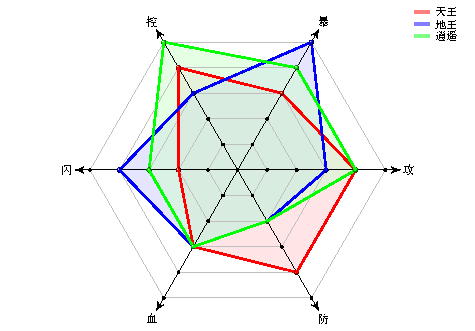
\includegraphics[width=0.8\textwidth]{radar7} 
\end{center}

\newpage
\section{辅助命令}
\subsection{维度坐标轴刻度值}  
\subsubsection{坐标轴刻度值命令}
\begin{NewMacroBox}{tkzRadarGrad}{\oarg{选项}\varp{整数}}
\begin{tabular}{lll}
必选参数 & 样例 & 含义                              \\ 
\midrule
\TAline{整数} {1}  {坐标轴维度编号}   
\end{tabular} 

\medskip
\begin{tabular}{lll}
可选参数 & 默认值 & 含义               \\
\midrule
\TOline{graduation distance}{0pt}{刻度值距坐标轴的垂直距离}
\TOline{prefix}   {empty} {刻度值数值前缀}
\TOline{suffix}   {empty} {刻度值数值后缀} 
\TOline{unity}   {1} {刻度值递增单位}
\bottomrule
\end{tabular} 

\emph{使用\tkzname{suffix}和\tkzname{prefix}的示例如下。}

\end{NewMacroBox}  

\subsubsection{为网格添加坐标轴刻度}  
\begin{tkzexample}[]
  \begin{tikzpicture}
    \tkzRadarDiagram[scale   = .8,
                     gap     = 1,  
                     lattice = 5]%
                     {天, 地, 人, 法, 器}
    \tkzRadarGrad[prefix=,unity=0.1,suffix=](1)  
  \end{tikzpicture}
\end{tkzexample}

\subsubsection{使用\tkzname{suffix}}  
\begin{tkzexample}[]
  \begin{tikzpicture}
    \tkzRadarDiagram[scale   = .8,
                     gap     = 1,  
                     lattice = 5]%
                     {天, 地, 人, 法, 器}
    \tkzRadarLine[thick,
                  color=blue,
                  mark=none,
                  fill=blue!20,
                  opacity=.5](3,3.5,3,3.5,3)
    \tkzRadarLine[thick,
                  color=darkgray,
                  fill=green!20,
                  opacity=.5](0.5,1,0.5,0.75,1) 
    \tkzRadarLine[ultra thick,
                  mark=ball,
                  mark size=4pt,
                  color =Maroon](2,3.75,1,1.5,2)    

    \tkzRadarGrad[prefix=,unity=100,suffix=\ \textyen](1)  
  \end{tikzpicture}
\end{tkzexample}
   

\subsubsection{使用\tkzname{prefix}}  
\begin{tkzexample}[]
  \begin{tikzpicture}[rotate=30, scale=.75]
    \tkzRadarDiagram[lattice = 6,
                     gap = 1,
                     step = 2,
                     label space = 2]%
                     {市场, 销售, 管理, 信息, 售后, 开发}
                     
    \tkzRadarLine[thick,
                  color=red](2.25,2.5,0.6,1.2,1,1)
    \tkzRadarLine[thick,
                  color=blue](1,2,1,1.7,1.3,3)

    \tkzRadarGrad[prefix=\$,unity=10](5)
  \end{tikzpicture}
\end{tkzexample}

\subsection{为雷达图添加图例}  
\subsubsection{添加图例命令}
\begin{NewMacroBox}{tkzLegendBox}{\oarg{选项}\varp{位置参数}\varp{图例参数}}
\begin{tabular}{lll}
必选参数 & 默认值 & 样例                              \\ 
\midrule
\TAline{位置参数} {空}  {相对于雷达图的位置}
\TAline{图例参数} {空}  {每个数据线的颜色及名称``颜色/名称''}
\end{tabular} 

\medskip
\begin{tabular}{lll}
可选参数 & 默认值 & 含义               \\
\midrule
\TOline{shift={}}{无}{位置偏移量}
\bottomrule
\end{tabular}
\end{NewMacroBox}  

\subsubsection{雷达图图例样例}  
\begin{tkzexample}[]
  \begin{tikzpicture}
   \begin{scope}  
    \tkzRadarDiagram[
           lattice=5,
           radial  style/.style ={-},% 不需要维度坐标轴箭头
           lattice style/.style ={blue!30}
          ]%
          {攻, 暴, 控, 闪, 血, 防}

    \tkzRadarLine[
           thick,
           color=red,
           mark=ball,
           ball color=red,
           mark size=4pt,
           fill=red!20](4, 3, 4, 2, 3, 4)

    \tkzRadarLine[
           thick,
           color=blue,
           mark=ball,
           mark size=4pt,
           fill=blue!20,opacity=.5](3, 5, 3, 4, 3, 2)
  \end{scope}

  \begin{scope}[scale = 0.8, every node/.append style = {transform shape}]
  \tkzLegendBox[shift={(-2.5cm,5.5cm)}]{current bounding box.south east}%
             {red/天王,
               blue/天忍}
  \end{scope} 
 \end{tikzpicture}
\end{tkzexample}


\clearpage
\newpage
\printindex
\end{document}


%%% Local Variables:
%%% mode: latex
%%% TeX-master: t
%%% End:

